\section{Vertex Reconstruction}\label{section:star_vertex}
When the charged-particle multiplicity is low, the vertex-finding algorithm sometimes fails to find the~primary vertex. In addition, at high luminosity, vertex finder can fail due to the contribution of pile-up interactions,  providing a wrong reconstructed vertex. In the study of vertex reconstruction efficiency we required at least two reconstructed global tracks $n^\textrm{global}_\textrm{sel}\geq 2$ passing all the quality cuts listed in Sec~\ref{section:star_track_selection}, except vertex-related cuts on $\textrm{DCA}_{xy}$ and $\textrm{DCA}_{z}$,  and  associated to true-level primary particles.  Additionally, MC events were accepted if the~$z$-coordinate of the~true-level primary vertex was between $-80$ and $80$~cm and $n_\textrm{ch}\geq 2$. All corrections, described in this section, were calculated in three ranges of $\xi$ separately using PYTHIA~8 \ac{SD} embedding \ac{MC}.

%\subsubsection{Track Quality Cuts Used for Vertexing}
The global tracks (not necessarily associated to a~true-level primary particles), which are used by the~vertex-finder algorithm, had to pass the~following quality cuts:
%The following quality cuts had to be passed by the global tracks (not necessarily associated to a~true-level primary particles) used by the~vertex-finder algorithm:% to used in the vertex reconstruction:
\begin{enumerate}
	\item tracks must be matched with hits reconstructed in TOF,
	\item the number of the TPC hits used in the helix fit $N_\textrm{hits}^\textrm{fit}$ must be greater than 20,
	\item the ratio of the number of TPC hits used in the helix fit to the number of possible TPC hits $N_\textrm{hits}^\textrm{fit}/N_\textrm{hits}^\textrm{poss}$ must be greater than $0.52$,
	\item the transverse impact parameter with respect to the beamline $d_0$ must be less than 2 cm,
	\item the track's transverse momentum $p_\textrm{T}$ must be greater than $0.2$~GeV/c.
\end{enumerate}



The~above track selection criteria are different than those used in the~nominal analysis. Primary vertex reconstruction efficiency and fake vertex rate were calculated as a function of the~number of global tracks used in vertexing $n^\textrm{global}_\textrm{vrt}$ instead of $n^\textrm{global}_\textrm{sel}$ ($n^\textrm{global}_\textrm{vrt}\geq n^\textrm{global}_\textrm{sel}$). 



%\subsubsection{Vertex Efficiency and Fake Vertex Rate}
In the~nominal analysis exactly one vertex with $n_\textrm{sel}\geq 2$ is required.  However, in the~study of vertex reconstruction, events with additional vertices were studied. Therefore, we define the~best vertex as the~reconstructed vertex with the highest number of TOF-matched tracks. This vertex does not have to be associated to true-level primary vertex (fake or secondary vertex). The algorithm, which matches reconstructed vertices to true-level vertices,  checks for reconstructed tracks originating from them. If at least one reconstructed track  is assigned to a true-level particle, then the reconstructed vertex is assigned to the true-level vertex from which the true-level particle originates. Since the~fake vertices (not matched to the true-level primary vertex) are allowed in the analysis, the~overall vertex-finding efficiency, $\epsilon_\textrm{vrt}\left(n_\textrm{vrt}^\textrm{global}\right)$, is expressed as:
\begin{equation}
\epsilon_\textrm{vrt}\left(n_\textrm{vrt}^\textrm{global}\right)=\epsilon_\textrm{vrt}^\textrm{best}\left(n_\textrm{vrt}^\textrm{global}\right)+\delta_\textrm{vrt}^\textrm{fake}\left(n_\textrm{vrt}^\textrm{global}\right)
\end{equation}
where:
\begin{description}
	\item $\epsilon_\textrm{vrt}^\textrm{best}\left(n_\textrm{vrt}^\textrm{global}\right)$ is the primary vertex reconstruction efficiency, determined as the ratio of the~number of good reconstructed events (best primary vertex with $n_\textrm{sel}\geq 2$ matched to the~true-level primary vertex) to the number of input MC events,
	\item $\delta_\textrm{vrt}^\textrm{fake}\left(n_\textrm{vrt}^\textrm{global}\right)$ is the fake vertex rate, determined as the ratio of the number of good reconstructed events (best primary vertex with $n_\textrm{sel}\geq 2$  not matched to the true-level primary vertex) to the number of input MC events. Due to the~contribution of pile-up, it is possible that the~best vertex originates from fake tracks instead of true-level particles.
\end{description}
\begin{comment}
\begin{figure}[b!]
\centering
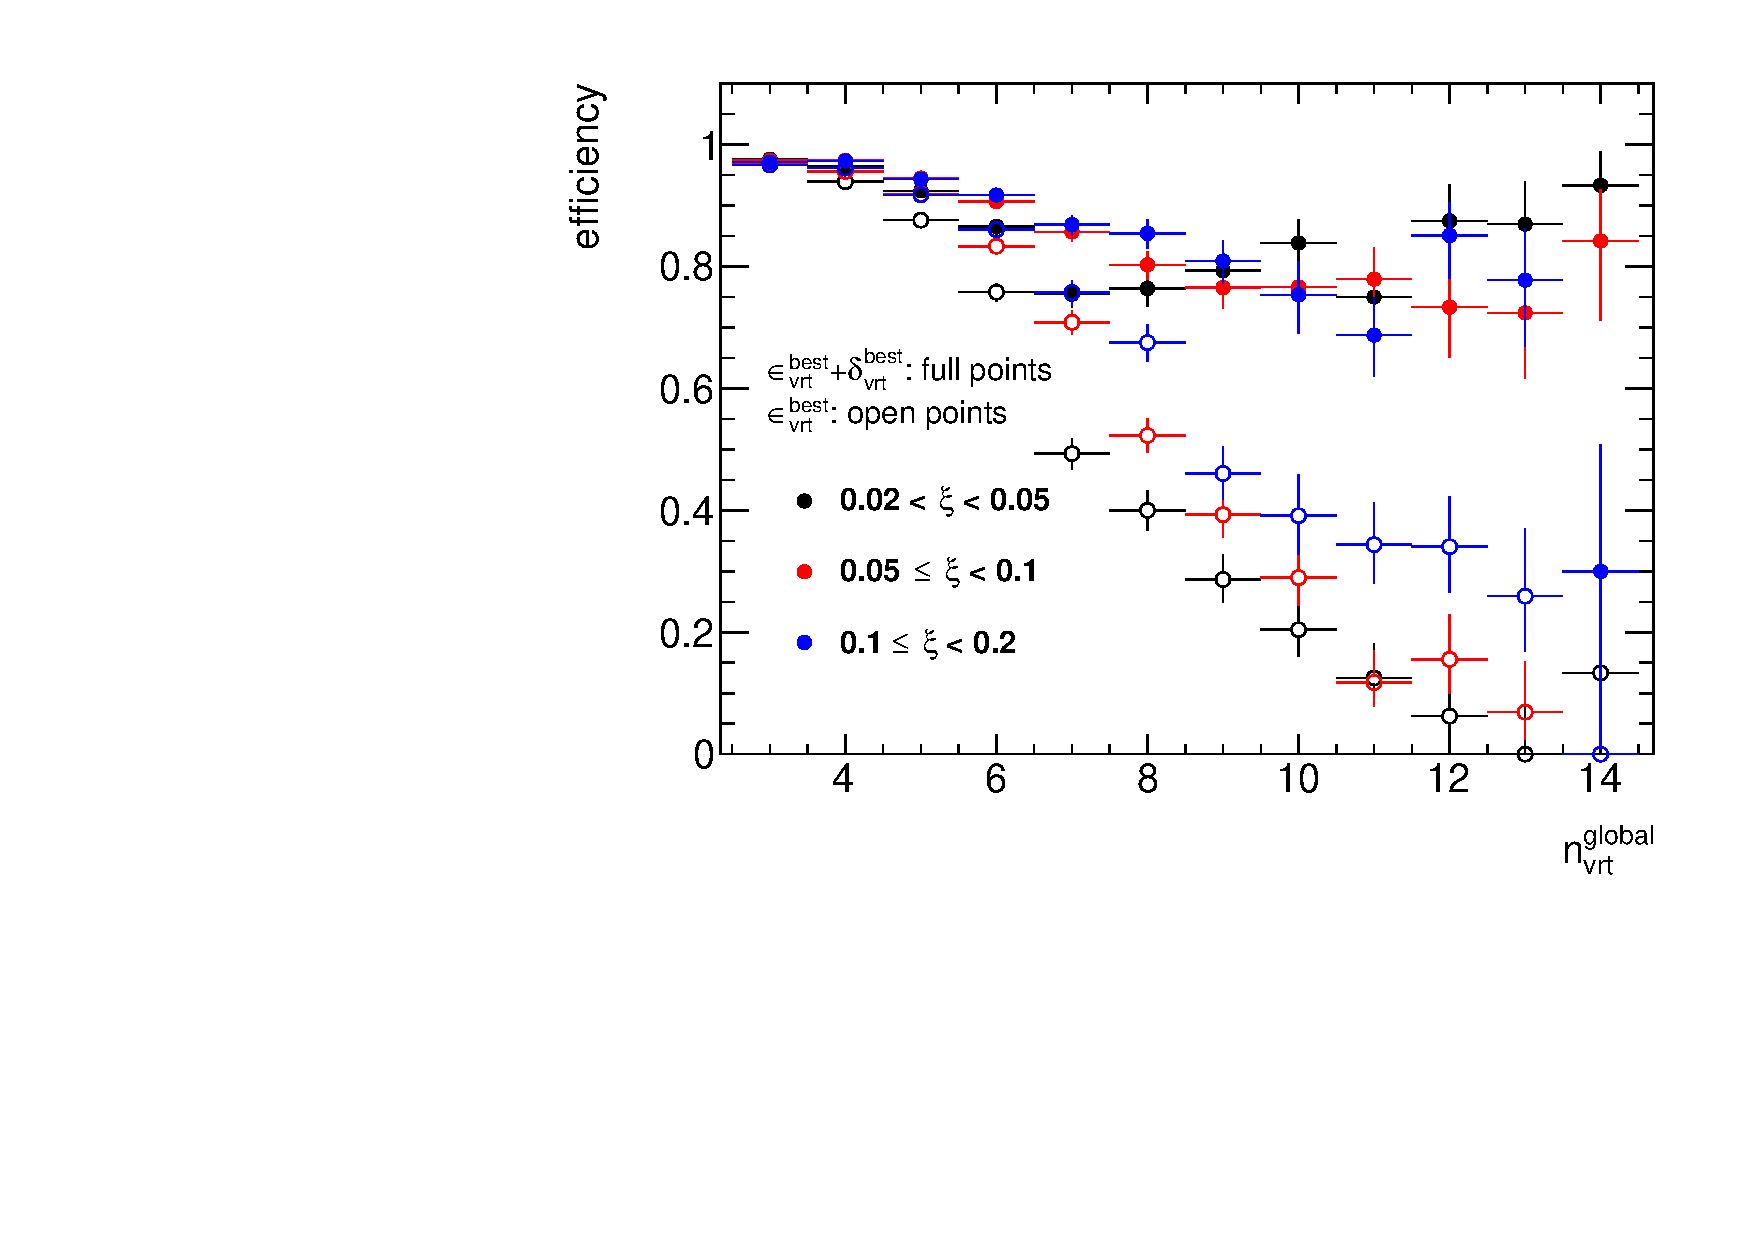
\includegraphics[width=0.49\textwidth,page=1]{chapters/chrgSTAR/img/vertex/vertexEffi_ksi.pdf}
\includegraphics[width=0.49\textwidth,page=8]{chapters/chrgSTAR/img/vertex/vertexEffi_ksi.pdf}
\caption{Vertex-finding efficiency in three ranges of $\xi$ as a function of  (left) $n^\textrm{global}_\textrm{vrt}$ and (right) with respect to the $|\Delta z_0|$ between reconstructed tracks in events with $n^\textrm{global}_\textrm{vrt}=2$. }
\label{fig:vertexEffi}
\end{figure}
\end{comment}
The vertex-finding efficiency as a function of $n^\textrm{global}_\textrm{vrt}$, shown in  Fig.~\ref{fig:vertexEffi}~(left), is larger than $75\%$ for all $n^\textrm{global}_\textrm{vrt}$. However, for $n^\textrm{global}_\textrm{vrt}>8$, there are more fake  than true-level primary vertices. When there are exactly two global tracks used in the vertex reconstruction, $n^\textrm{global}_\textrm{vrt}=2$, the vertex-finding efficiency depends on the longitudinal distance between these tracks $|\Delta z_0|$. Therefore, the~vertex-finding efficiency for such events $\epsilon_\textrm{vrt}\left(|\Delta z_0|\right)$ is given by:
\begin{equation}
\epsilon_\textrm{vrt}\left(|\Delta z_0|\right)=\epsilon_\textrm{vrt}^\textrm{best}\left(|\Delta z_0|\right)+\delta_\textrm{vrt}^\textrm{fake}\left(|\Delta z_0|\right)
\end{equation}
where: $\epsilon_\textrm{vrt}^\textrm{best}\left(|\Delta z_0|\right)$ is the primary vertex reconstruction efficiency, $\delta_\textrm{vrt}^\textrm{fake}\left(|\Delta z_0|\right)$ is the fake vertex rate.

\begin{figure}[b!]
	\vspace{-0.4cm}
	\centering
	\begin{subfigure}{.49\textwidth}
		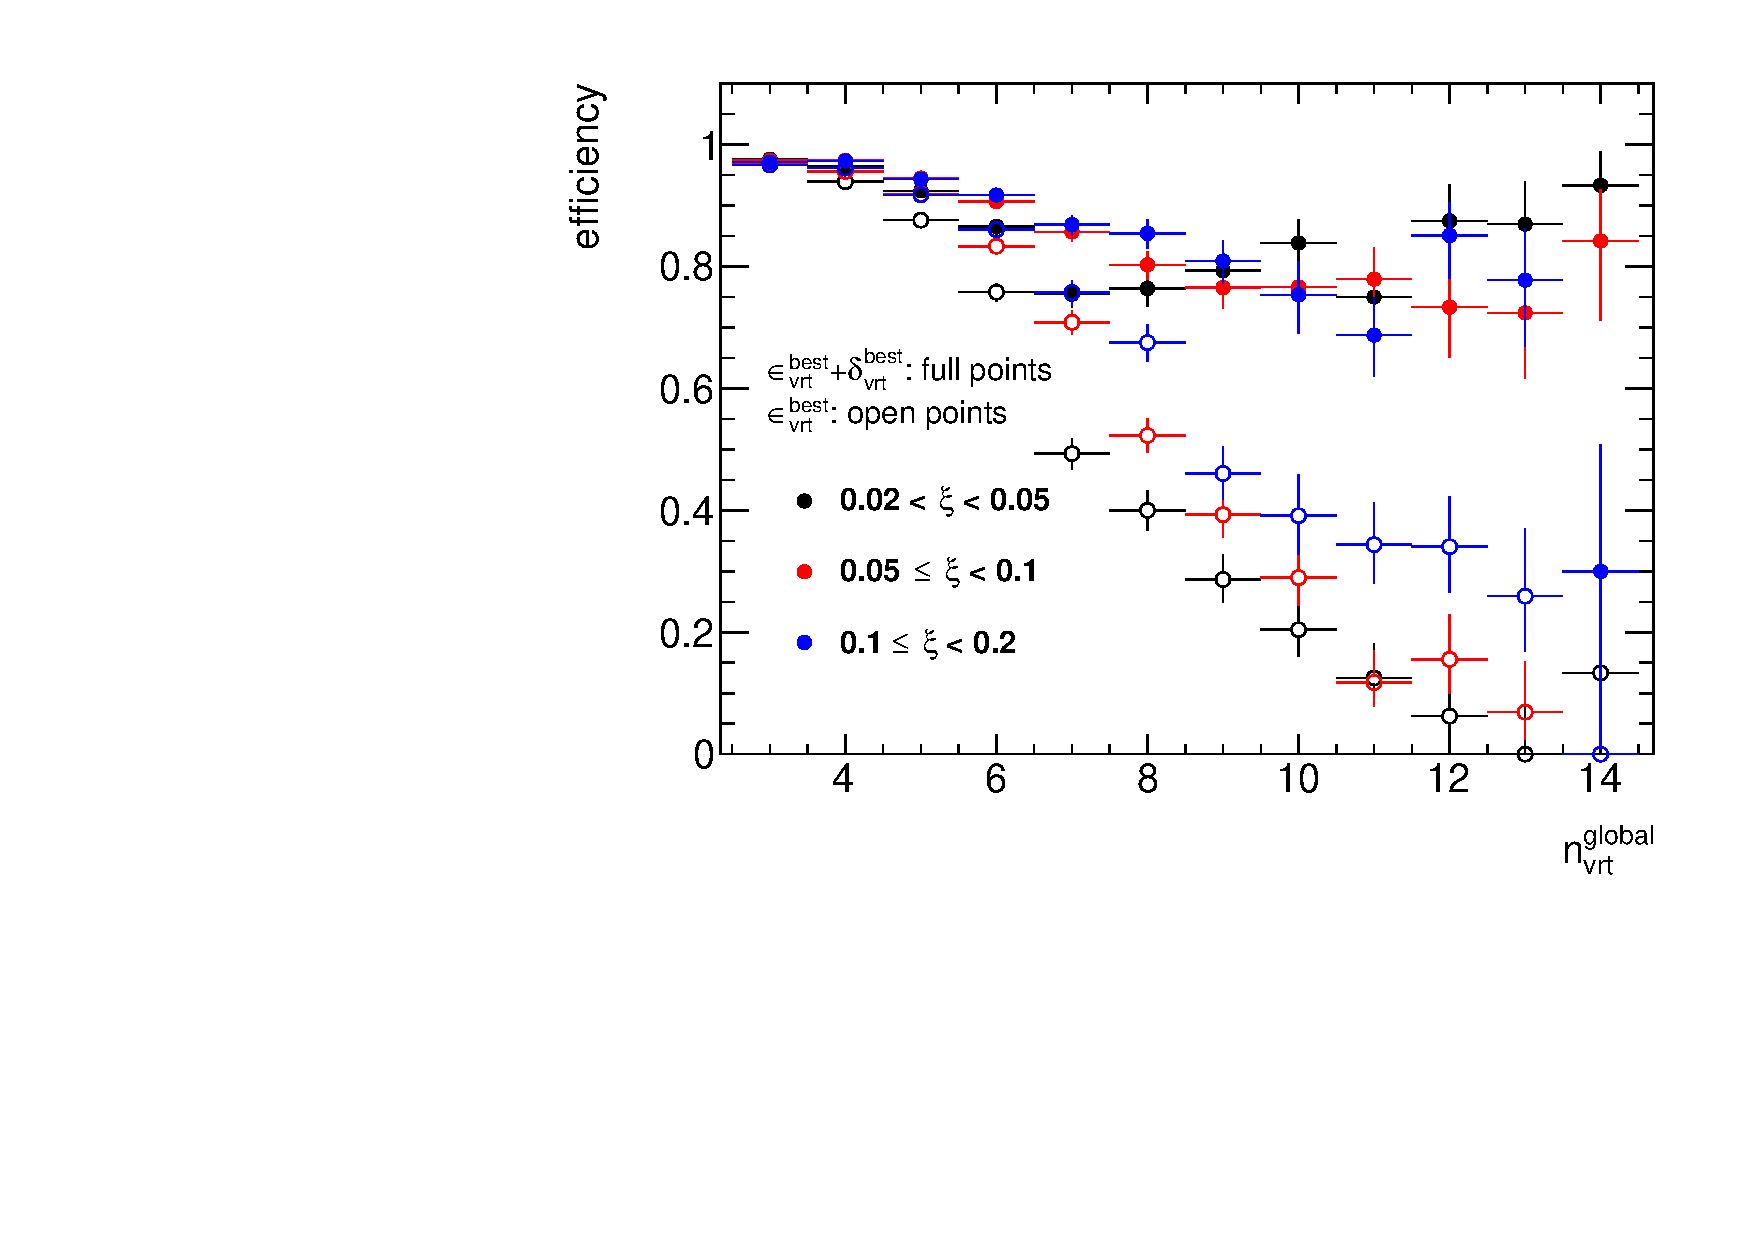
\includegraphics[width=1.0\textwidth,page=1]{chapters/chrgSTAR/img/vertex/vertexEffi_ksi.pdf}
	\end{subfigure}
	\begin{subfigure}{.49\textwidth}
		\includegraphics[width=1.0\textwidth,page=8]{chapters/chrgSTAR/img/vertex/vertexEffi_ksi.pdf}
	\end{subfigure}
	
	\vspace{-0.3cm}
	\caption{Vertex-finding efficiency in three ranges of $\xi$ as a function of  (left) $n^\textrm{global}_\textrm{vrt}$ and (right) with respect to the $|\Delta z_0|$ between reconstructed tracks in events with $n^\textrm{global}_\textrm{vrt}=2$. }
	\label{fig:vertexEffi}
\end{figure}

Figure~\ref{fig:vertexEffi}~(right) shows the vertex-finding efficiency for events with $n^\textrm{global}_\textrm{vrt}=2$. This efficiency is smaller than $20\%$ for tracks with $|\Delta z_0|>2$~cm, hence the analysis was limited to  events with  $|\Delta z_0|<2$~cm, when $n^\textrm{global}_\textrm{vrt}=2$.  The rate of fake vertices is negligibly low (open points overlap with full points).


%\subsubsection{Other Corrections to the Reconstructed Vertices}
%Events with reconstructed best vertex are rejected if there  are:
Events are rejected if more vertices are reconstructed in addition to the~best one. Rejected events can be classified as:

\begin{enumerate}[label=\alph*)]
	\item two or more additional vertices,
	\item additional  secondary vertex from interactions with the detector dead-material,
	\item additional fake  vertex,
	\item additional primary  vertex (vertex splitting or background vertex reconstructed as best vertex),
	\item additional secondary vertex from the decay. 
\end{enumerate}


\begin{figure}[b!]
	%\vspace{-1.cm}
	%\vspace{-0.4cm}
	\centering
	\begin{subfigure}{.49\textwidth}
		\includegraphics[width=\textwidth,page=3]{chapters/chrgSTAR/img/vertex/vertexEffi_ksi.pdf}
	\end{subfigure}
	\vspace{-0.1cm}
	\hfill
	\begin{subfigure}{.49\textwidth}
		\includegraphics[width=\textwidth,page=4]{chapters/chrgSTAR/img/vertex/vertexEffi_ksi.pdf}
	\end{subfigure}
	
	\begin{subfigure}{.49\textwidth}
		\includegraphics[width=\textwidth,page=5]{chapters/chrgSTAR/img/vertex/vertexEffi_ksi.pdf}
	\end{subfigure}
	\vspace{-0.1cm}
	\hfill
	\begin{subfigure}{.49\textwidth}
		\includegraphics[width=\textwidth,page=6]{chapters/chrgSTAR/img/vertex/vertexEffi_ksi.pdf}
	\end{subfigure}
	
	\begin{subfigure}{.49\textwidth}
		\includegraphics[width=\textwidth,page=7]{chapters/chrgSTAR/img/vertex/vertexEffi_ksi.pdf}
	\end{subfigure}
	\hfill
	\begin{minipage}{.47\textwidth}
		\caption{Fraction of multi-vertex events  with respect to the $n_\textrm{vrt}^\textrm{global}$ in three ranges of $\xi$. Each contribution is shown separately: (top left) more than one additional vertices, (top right) additional secondary vertex from the interactions with the detector dead-material, (middle left) additional fake vertex, (middle right) additional primary vertex and (bottom) additional decay vertex.}
		\label{fig:vertexVeto}
	\end{minipage}
	%\vspace{-0.7cm}
\end{figure}

The fraction of such events, $f_\textrm{vrt}^\textrm{veto}\left(n_\textrm{vrt}^\textrm{global}\right)$, is given by: 
\begin{equation}
\begin{split}
f_\textrm{vrt}^\textrm{veto}\left(n_\textrm{vrt}^\textrm{global}\right) & =\frac{\textrm{number of events with more than one reconstructed  TOF vertex}}{\textrm{number of events with at least one reconstructed TOF vertex}} \\
& =f_a+f_b+f_c+f_d+f_e
\end{split}
\label{eq:vertexVetoEq}
\end{equation}
where $f_a$ to $f_e$ are the fractions of events with additional vertices, with labels corresponding to the~items in the~listing above.% shown in \ref{fig:vertexVeto}.


%\newpage

\begin{figure}[t!]
	%\vspace{0.2cm}
	\centering
	\begin{subfigure}{.49\textwidth}
		\includegraphics[width=\textwidth,page=2]{chapters/chrgSTAR/img/vertex/vertexEffi_ksi.pdf}
	\end{subfigure}
	\begin{subfigure}{.49\textwidth}
		\includegraphics[width=\textwidth,page=9]{chapters/chrgSTAR/img/vertex/vertexEffi_ksi.pdf}
	\end{subfigure}
	\caption{Total fraction of multi-vertex events as a function of (left) $n_\textrm{vrt}^\textrm{global}$ for events with $n^\textrm{global}_\textrm{vrt}>2$ and (right) $|\Delta z_0|$ for events with $n^\textrm{global}_\textrm{vrt}=2$  in three ranges of $\xi$.}
	\label{fig:vertexVetoDZ}
	\vspace{0.5cm}
	%\end{figure}
	
	%\begin{figure}[t!]
	\begin{subfigure}{.46\textwidth}
		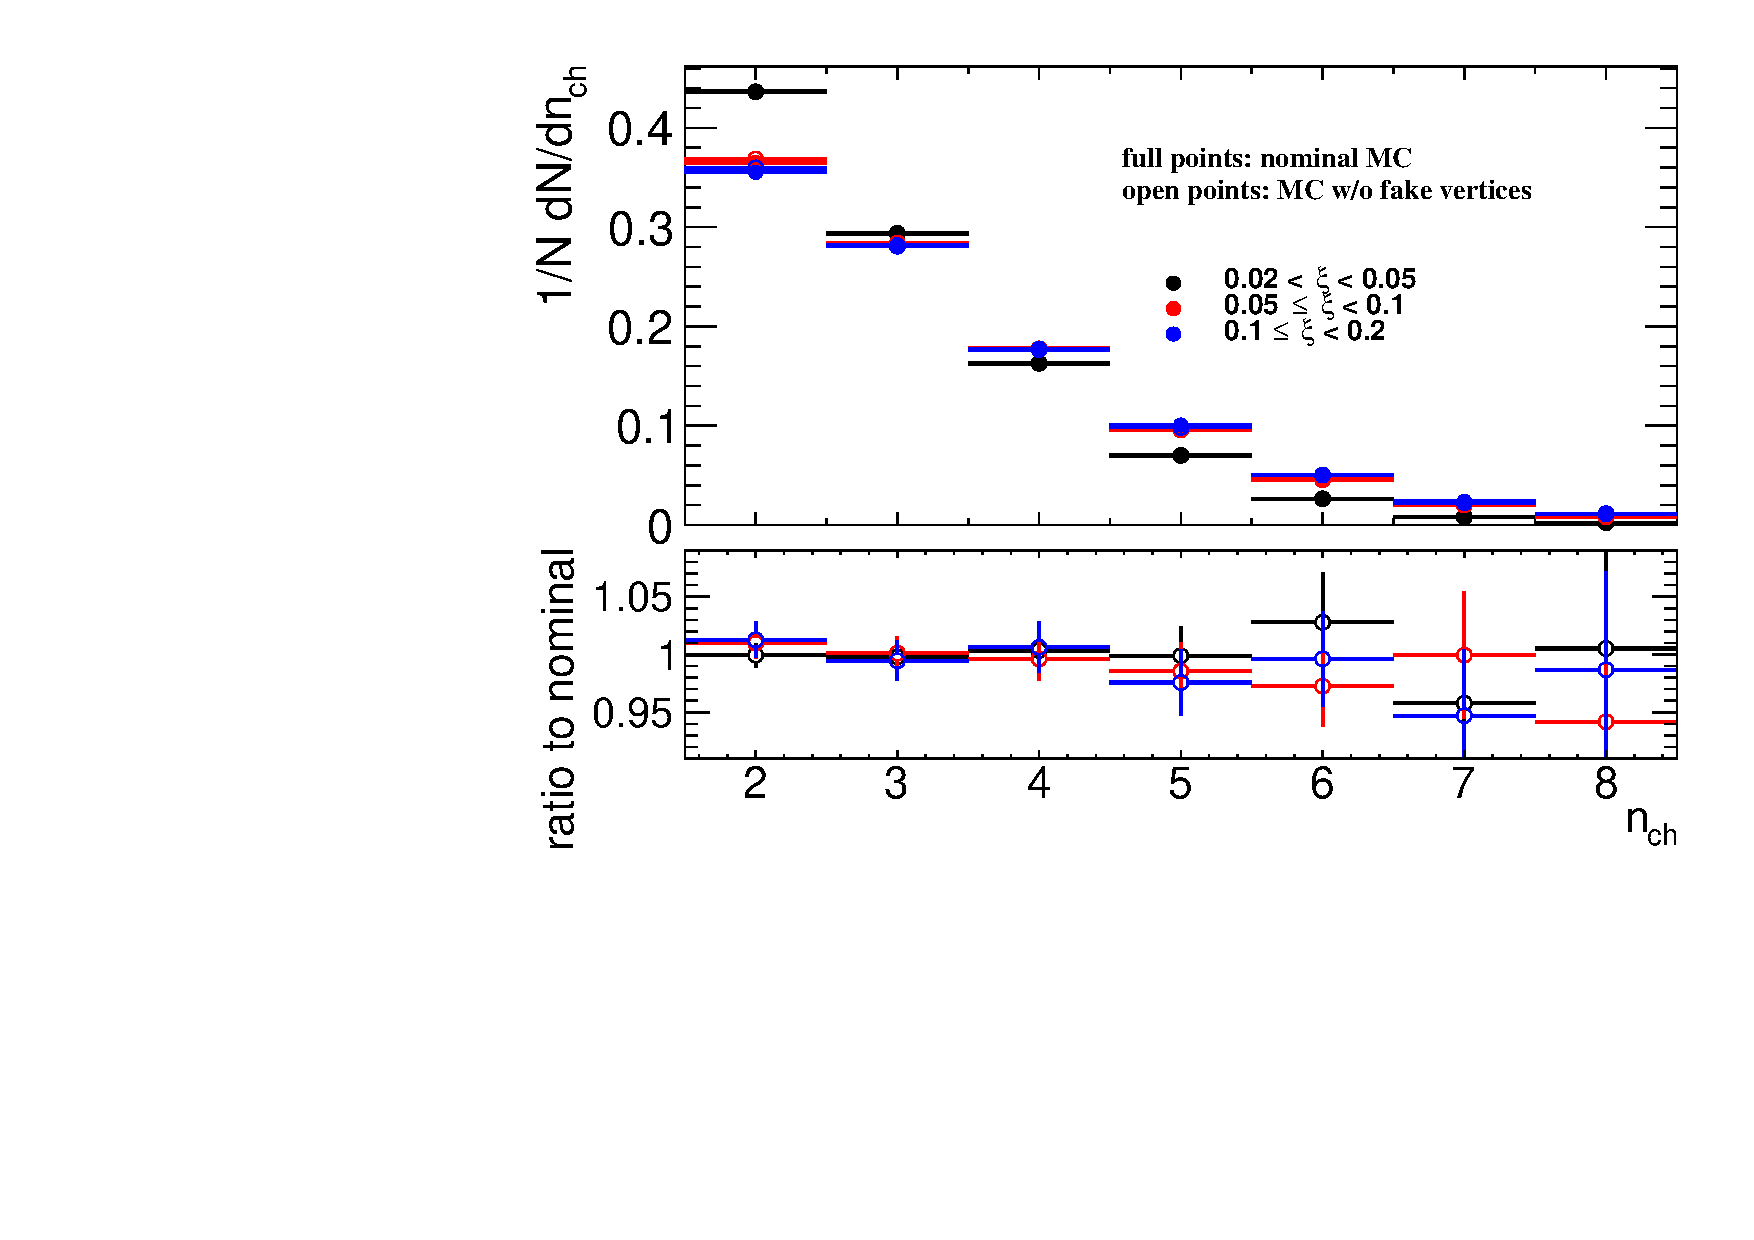
\includegraphics[width=\textwidth,page=1]{chapters/chrgSTAR/img/vertex/nchFake.pdf}
	\end{subfigure}
	\begin{minipage}{.47\textwidth}
		\hfill
		\begin{minipage}{0.95\textwidth}
			\caption{Normalized charged-particle multiplicity distributions in three ranges of $\xi$ calculated from PYTHIA~8 SD embedding  MC for (full points) all generated events and (open points) events without reconstructed fake vertices.}
			\label{fig:nchVertex}
		\end{minipage}
		
	\end{minipage}
	\vspace{1em}
	%\end{figure}
	
	%\begin{figure}[t!]
	\centering
	%\thispagestyle{empty}
	\begin{subfigure}{.49\textwidth}
		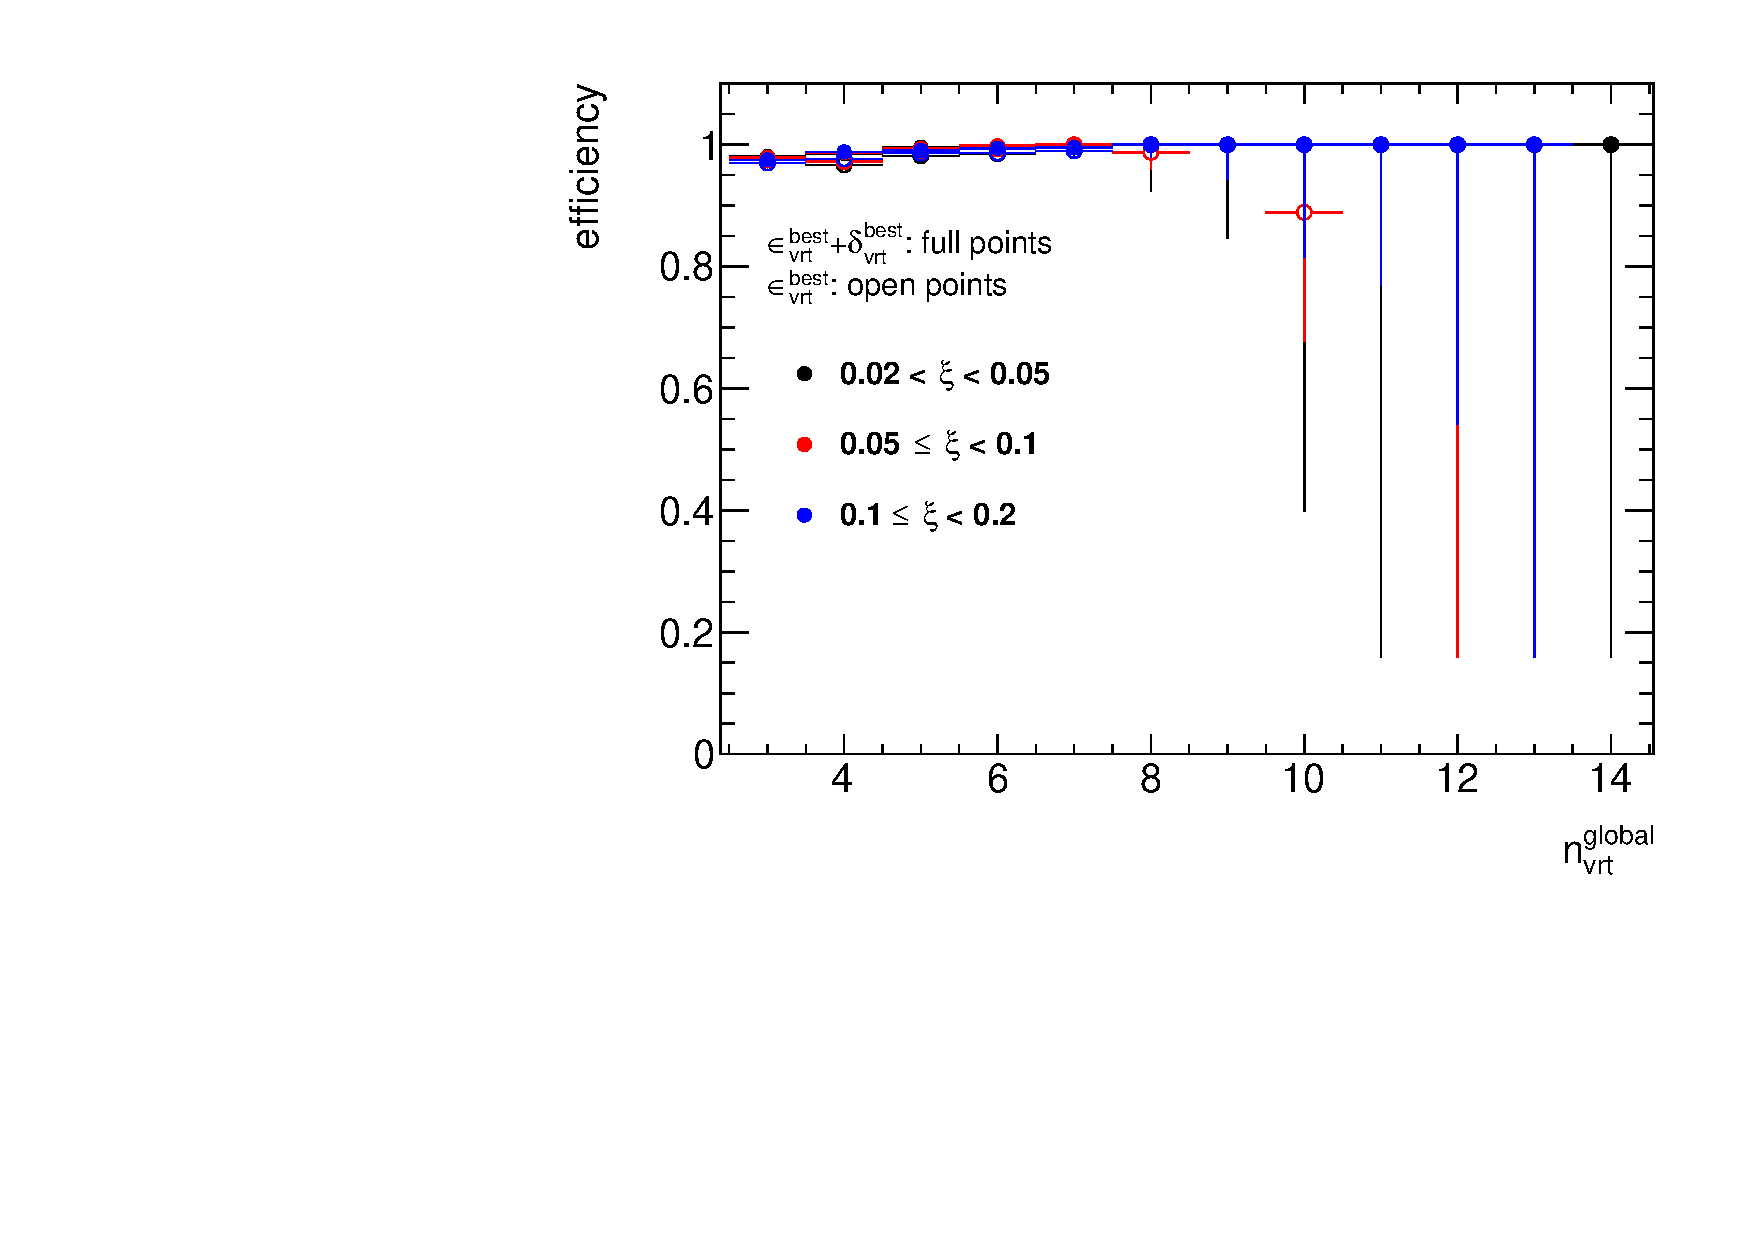
\includegraphics[width=\textwidth,page=1]{chapters/chrgSTAR/img/vertex/vertexEffi_ksi_noFake.pdf}
	\end{subfigure}
	\begin{subfigure}{.49\textwidth}
		\includegraphics[width=\textwidth,page=8]{chapters/chrgSTAR/img/vertex/vertexEffi_ksi_noFake.pdf}
	\end{subfigure}
	\caption{Vertex-finding efficiency in three ranges of $\xi$ as a~function of  (left) $n^\textrm{global}_\textrm{vrt}$ and (right) with respect to the $|\Delta z_0|$ between reconstructed tracks in events with $n^\textrm{global}_\textrm{vrt}=2$. Only events that do not contain additional fake vertices were used. }
	\label{fig:vertexEffi_noFake}
	%\vspace{1cm}
\end{figure}

As before, the fraction was calculated as a function of $|\Delta z_0|$ for events with $n^\textrm{global}_\textrm{vrt}=2$. Figure~ \ref{fig:vertexVeto} shows the fraction of multi-vertex events  with respect to the $n_\textrm{vrt}^\textrm{global}$. There is a~large fraction of events ($>90\%$) with additional background vertices for $n_\textrm{vrt}^\textrm{global}\geq 9$, what would result in large correction factor. Hence, the analysis was limited to events with $n_\textrm{sel}^\textrm{global}\leq8$ ($n_\textrm{sel}^\textrm{global}\leq n_\textrm{vrt}^\textrm{global}$). The total fraction of multi-vertex events, $f_a+f_b+f_c+f_d+f_e$, as a function of $n^\textrm{global}_\textrm{vrt}$ and $|\Delta z_0|$, shown in Fig.~\ref{fig:vertexVetoDZ}, demonstrates that $f_\textrm{vrt}^\textrm{veto}(|\Delta z_0|)$ is very small ($<2\%$) for events with $n^\textrm{global}_\textrm{vrt}=2$.



%\begin{figure}[b!]
%\vspace{-0.5cm}
%	\centering

%\vspace{-0.5cm}
%\end{figure}


\begin{figure}[b!]
	%\vspace{-0.3cm}
	\centering
	\begin{subfigure}{.49\textwidth}
		\includegraphics[width=\textwidth,page=3]{chapters/chrgSTAR/img/vertex/vertexEffi_ksi_noFake.pdf}
	\end{subfigure}
	%\vspace{-0.1cm}
	\begin{subfigure}{.49\textwidth}
		\includegraphics[width=\textwidth,page=4]{chapters/chrgSTAR/img/vertex/vertexEffi_ksi_noFake.pdf}
	\end{subfigure}
	\begin{subfigure}{.49\textwidth}
		\includegraphics[width=\textwidth,page=6]{chapters/chrgSTAR/img/vertex/vertexEffi_ksi_noFake.pdf}
	\end{subfigure}
	%\vspace{-0.2cm}
	\begin{subfigure}{.49\textwidth}
		\includegraphics[width=\textwidth,page=7]{chapters/chrgSTAR/img/vertex/vertexEffi_ksi_noFake.pdf}
	\end{subfigure}
	\caption{Fraction of multi-vertex events  with respect to the $n_\textrm{vrt}^\textrm{global}$ in three ranges of $\xi$. Each contribution is shown separately: (top left) more than one additional vertices, (top right) additional secondary vertex from the interactions with the detector dead-material, (bottom left) additional primary vertex and (bottom right)  additional decay vertex. Only events that do not contain additional fake vertices were used.}
	\label{fig:vertexVeto_noFake}
	%\vspace{1.cm}
	%\vspace{-0.5cm}
	%\end{figure}
\end{figure}

Although, the analysis was limited to $n_\textrm{sel}^\textrm{global}\leq8$ ($n_\textrm{sel}^\textrm{global}\leq n_\textrm{vrt}^\textrm{global}$), a~fraction  of events  with additional background vertices was still relatively large.
Since most of these additional vertices are fake (and as accidental not correlated with true-level primary distributions), it was checked whether the~charged-particle multiplicity distributions are different for events with and without reconstructed fake vertices. These distributions, as shown in Fig~\ref{fig:nchVertex}, are in good agreement, thus, above studies of vertex reconstruction were repeated using \ac{MC} events that do not contain reconstructed fake vertices. It means that events with additional fake vertex  were rejected (similarly to the analysis of real data) and no correction is needed for such losses  since it only affects overall normalization (not the shapes of distributions under study). The~vertex-finding efficiency, which was  calculated from such events, is shown in Fig.~\ref{fig:vertexEffi_noFake}. It is greater than $95\%$ for events with $2 \leq n_\textrm{vrt}^\textrm{global}\leq 8$. 
In addition, the~corresponding fraction of multi-vertex events, shown in \cref{fig:vertexVetoDZ_noFake,fig:vertexVeto_noFake}, is smaller than $20\%$. Since fake vertices were rejected from this study, the~$f_{c}$ term from Eq.~\eqref{eq:vertexVetoEq} is equal to $0$. The~correction factors calculated from \ac{MC} events that do not contain reconstructed fake vertices  were used in the analysis instead of the~one obtained from the~full \ac{MC} sample.








\begin{figure}[b!]
	\thisfloatpagestyle{fancy}
	%\vspace{-0.5cm}
	\centering
	\begin{subfigure}{.49\textwidth}
		\includegraphics[width=\textwidth,page=2]{chapters/chrgSTAR/img/vertex/vertexEffi_ksi_noFake.pdf}
	\end{subfigure}
	%\vspace{-0.3cm}
	\begin{subfigure}{.49\textwidth}
		\includegraphics[width=\textwidth,page=9]{chapters/chrgSTAR/img/vertex/vertexEffi_ksi_noFake.pdf}
	\end{subfigure}
	\vspace{-0.2cm}
	\caption{Total fraction of multi-vertex events as a function of (left) $n_\textrm{vrt}^\textrm{global}$ for events with $n^\textrm{global}_\textrm{vrt}>2$ and (right) $|\Delta z_0|$ for events with $n^\textrm{global}_\textrm{vrt}=2$  in three ranges of $\xi$. Only events that do not contain additional fake vertices were used. }
	\label{fig:vertexVetoDZ_noFake}
	%\vspace{-0.2cm}
\end{figure}

\FloatBarrier
